\section{Funcionamiento}
	La figura \ref*{figInitialState} muestra el estado de la aplicación al abrir, lso agentes se colocan de manera aleatoria en el entorno, para colocar los objetos, en el menú superior se encuentran las opciones. Para colocar un objeto basta con dar click en la opción deseada y luego dar click en el tablero.
	
	Una vez se colocan todos los elementos la aplicación luce como en la figura \ref*{figSetUp}, luego se selecciona la opción de \textit{file} en el menú superior y se da click en \textit{run} para que los agentes desarrollen su tarea.
	
	Cuando un agente tiene una muestra se dirige a la nave por la distancia más corta, como se muestra en la figura \ref*{figSample} saltándose cualquier otra muestra que pueda estar en el camino. Una ver terminado el tablero queda sin muestras (figura \ref*{figEnd}).
	
	\begin{multicols}{2}
		\begin{figure}[H]
			\centering
			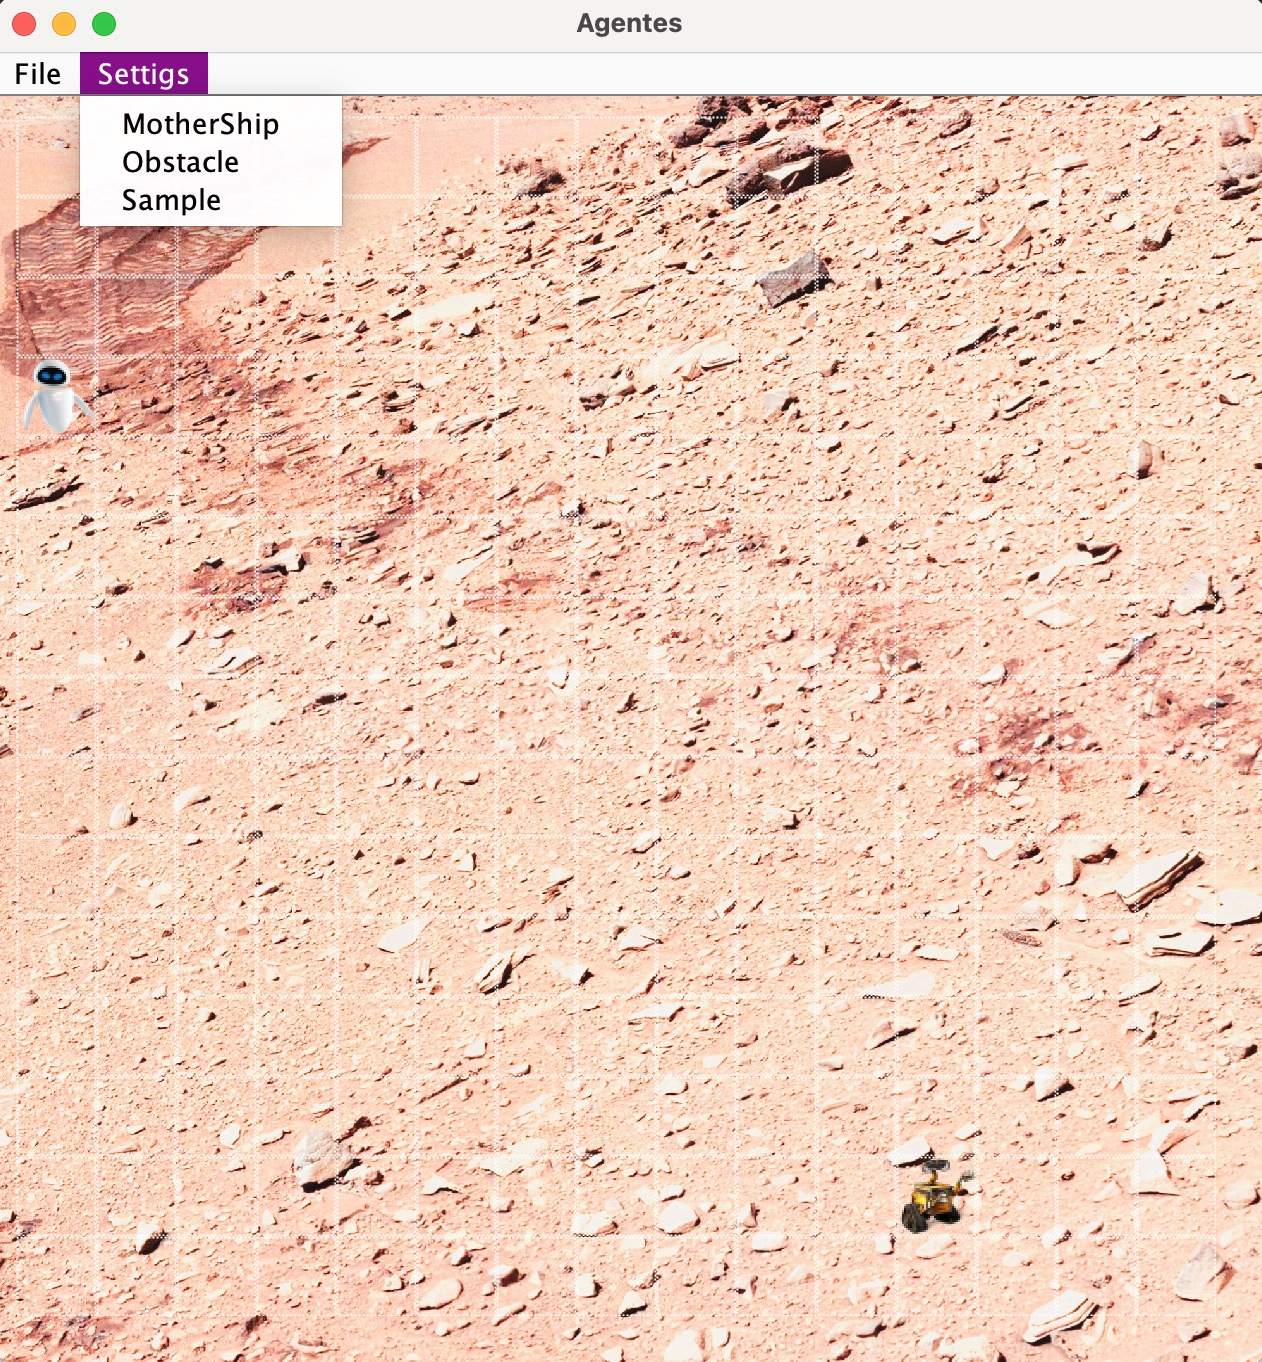
\includegraphics[width = 5cm]{images/initialState.jpg}
			\caption{Estado inicial de la aplicación.}
			\label{figInitialState}
		\end{figure}
		
	
		\begin{figure}[H]
			\centering
			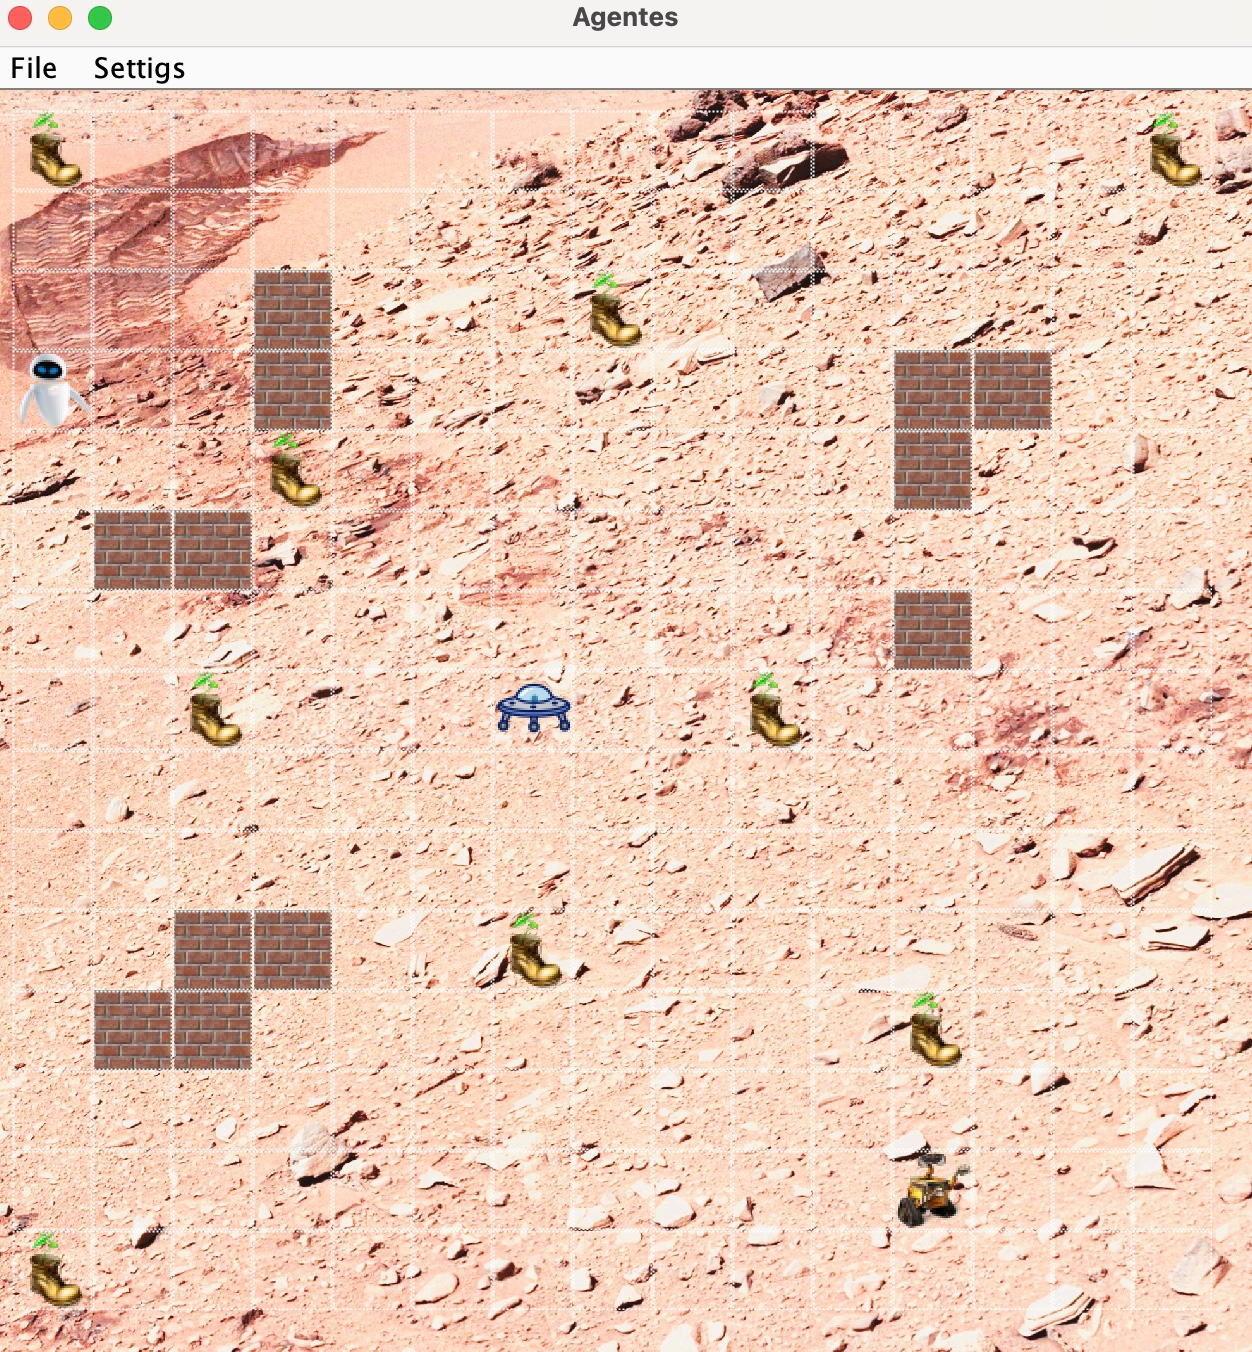
\includegraphics[width = 5cm]{images/setUp.jpg}
			\caption{Se configuró el entorno agregando la nave, las muestras y los obstáculos.}
			\label{figSetUp}
		\end{figure}
		
		\begin{figure}[H]
			\centering
			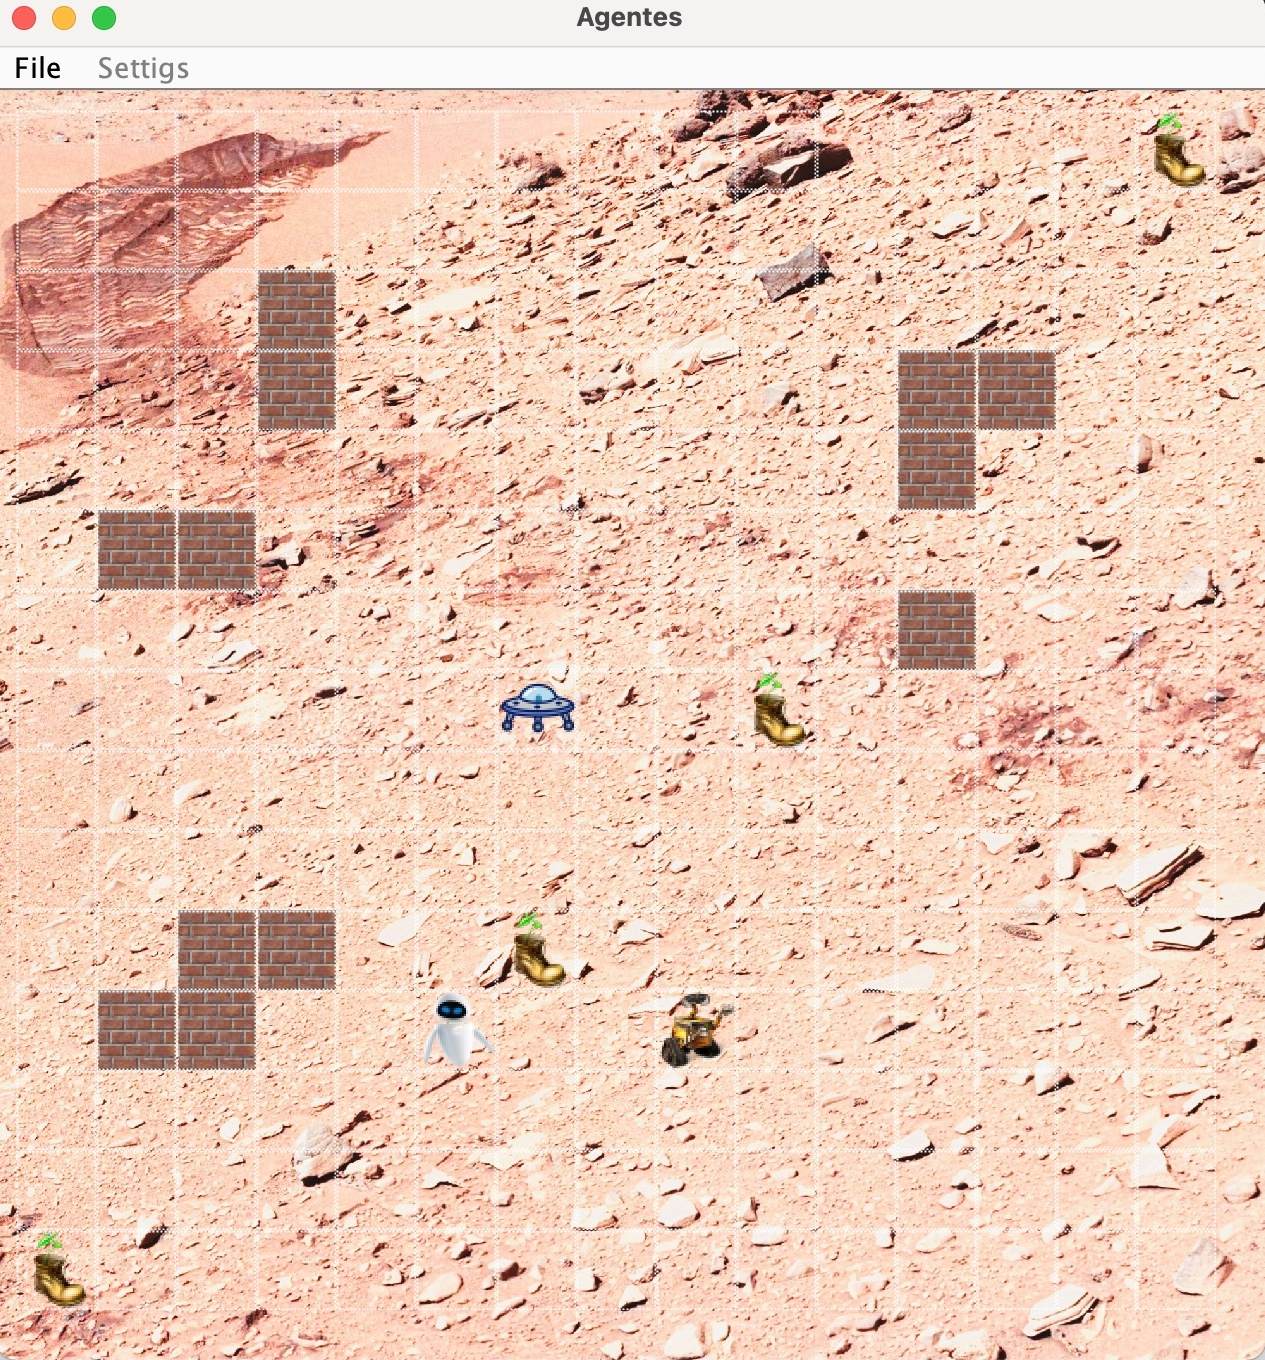
\includegraphics[width = 5cm]{images/sample.jpg}
			\caption{El agente dos se dirige a la nave por la distancia \textit{manhattan} más corta.}
			\label{figSample}
		\end{figure}
		\begin{figure}[H]
			\centering
			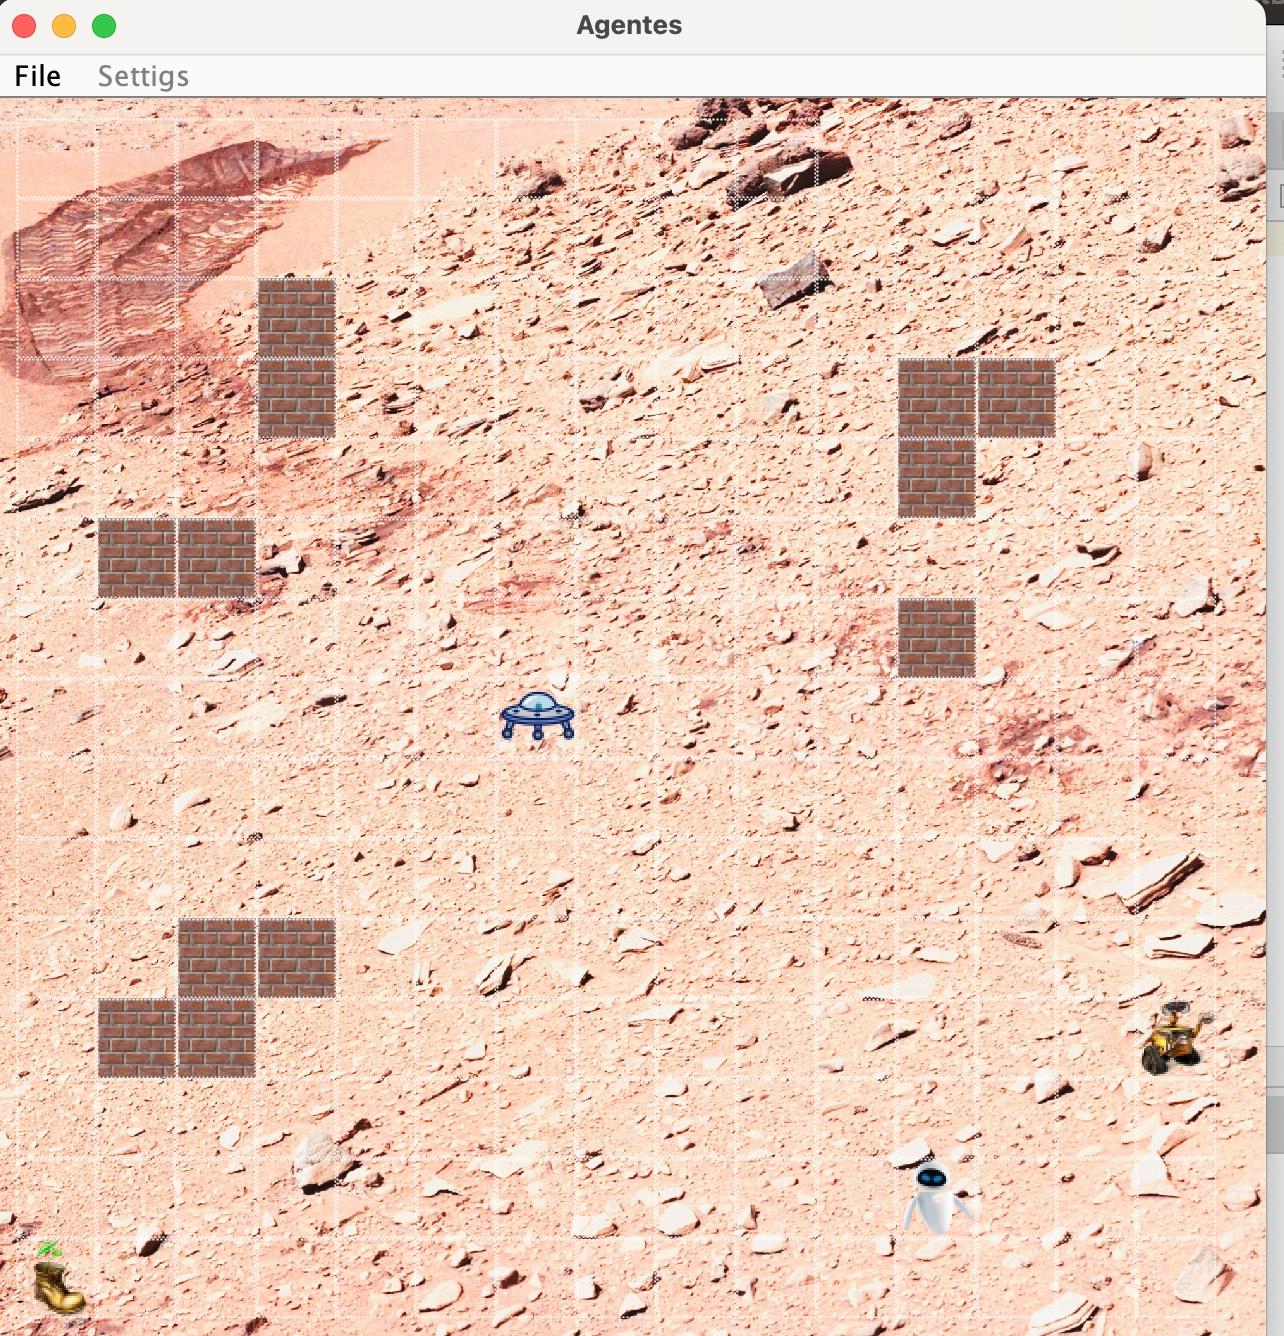
\includegraphics[width = 5cm]{images/end.jpg}
			\caption{Los agentes recolectaron todas las muestras.}
			\label{figEnd}
		\end{figure}
	\end{multicols}